\title{Lecture 18\\Representation of Processes and Actions in a Knowledge Base}

\begin{frame}
	\titlepage
\end{frame}

\begin{frame}{\\Lecture outline}
	\topline
	\justifying
	Processes, influences, and actions. Describing actions and elementary events in semantic memory. Classifying actions, including those performed in semantic memory. Relations on the set of actions. The context of action execution. Initial and final situations of a process.
\end{frame}

\begin{frame}{\\The concept of a process}
\topline
\justifying
\begin{SCn}
	\scnheader{structure}
	\begin{scnrelfromset}{partition}
		\scnitem{process}
		\begin{scnindent}
			\scnidtf{dynamic structure}
			\scnidtf{non-stationary structure}
		\end{scnindent}
		\scnitem{static structure}
		\begin{scnindent}
			\scnidtf{stationary structure}
			\scnidtf{structure that does not change over time}
		\end{scnindent}
	\end{scnrelfromset}
\end{SCn}

In OSTIS systems, a process is the transformation of a temporal entity from one state to another (a transition from one situation to another).
\end{frame}

\begin{frame}{\\The concept of a process}
\topline
\justifying

    Each \textbf{\textit{process}} is defined by the appearance or disappearance of connections between the given \textit{temporal entity} and other entities, and between parts of that temporal entity and other entities.\\
    Many \textit{\textbf{processes}} can be associated with an \textit{initial situation*} and a \textit{final situation*} (the situations between which the process makes the transition).\\
    \bigskip
    \textit{A process} is a dynamic structure that changes over time and generally cannot be represented in full in a knowledge base. An sc-element can, however, denote a particular process, with a description of its decomposition into more specific processes or of the situations corresponding to its states at different times.
\end{frame}

\begin{frame}{\\The concept of influence}
\topline
\justifying

 \begin{SCn}
	\scnheader{influence}
	\scnidtf{\textit{process} in which one entity (or a set of \textit{entities}) affects another \textit{entity} (or a set of other \textit{entities})}
	\scnidtf{\textit{process} in which at least one influencing entity (the \textit{subject\scnrolesign}) and at least one \textit{entity} being influenced (the \textit{object\scnrolesign})}
	\scnidtf{act of influence}
	\scnsubset{process}
	\begin{scnindent}
		\scnidtf{dynamic structure}
	\end{scnindent}

\end{SCn}
\end{frame}

\begin{frame}{\\Participants in an influence}
\topline
\justifying
\begin{SCn}
    \scnheader{subject}
	\scnidtf{active entity}
	\scnsubset{entity}
	\scnidtftext{frequently used sc-identifier}{individual}

    \scnheader{subject\scnrolesign}
	\scnidtf{influencing entity\scnrolesign}
	\scnidtf{entity that \textit{causes} a change in another entity (the object)\scnrolesign}

	\scnheader{object\scnrolesign}
	\scnidtf{entity being influenced\scnrolesign}
	\scnidtf{entity that serves as the initial condition (argument) necessary for the given influence\scnrolesign}
\end{SCn}
\end{frame}

\begin{frame}{}
\topline
\justifying
    Every \textit{influence} may be associated with (1) a \textit{subject\scnrolesign}, the entity exerting it (which may, for example, be a physical field), and (2) an \textit{object\scnrolesign}, the entity toward which it is directed. If the \textit{influence} concerns a \textit{material entity}, the object is that material entity or one of its spatial parts.
\end{frame}

\begin{frame}{}
\topline
\justifying

Since \textit{influences} are a type of \textit{process}, they inherit all properties of processes. This includes \textit{parameters} and \textit{relations} defined on processes, such as \textit{duration\scnsupergroupsign}, \textit{initial situation*}, and \textit{final situation*}.

\bigskip

An influence is a process and therefore a \textit{dynamic structure}. The signs of the \textit{subject of influence\scnrolesign} and the \textit{object of influence\scnrolesign} are both elements of that structure. The corresponding relations can therefore be treated as \textit{role relations}. Introducing analogous \textit{non-role relations} is possible but offers no practical benefit.
\end{frame}

\begin{frame}{\\The concept of an action}
\topline
\justifying
	\setlength{\emergencystretch}{2em}
\vspace{10mm}
 \begin{SCn}
	\scnheader{action}
	\scnidtf{\textit{influence} that a \textit{subject\scnrolesign} exerts deliberately in accordance with a \textit{goal*}}
	\scnidtf{goal-directed influence exerted by one or more subjects (cybernetic systems), possibly using tools}
	\scnidtf{act}
	\scnidtf{operation}
	\scnidtf{deliberate influence}
	\scnidtf{active influence}
	\scnsubset{influence}
	\begin{scnindent}
		\scnsubset{process}
	\end{scnindent}
 \scnidtf{goal-directed (\scnqq{deliberate}) process performed, controlled, or implemented by a subject}
\end{SCn}
\end{frame}

\begin{frame}{}
\begin{SCn}
	\scnidtf{work}
	\scnidtf{process of solving a problem}
	\scnidtf{process of achieving a goal}
	\scnidtf{coherent fragment of an activity}
	\scnidtf{goal-directed process controlled by a subject}
	\scnidtf{process in which a subject (performer) carries out an action on one or more objects}

	\scnheader{goal*}
	\scnidtf{goal situation*}
	\scnsubset{specification*}
	\scnidtf{description of what must be obtained, or which situation must be reached, by carrying out the specified action*}
\end{SCn}
\end{frame}

\begin{frame}{}
\justifying
\vspace{10mm}
Each \textit{action} performed by a \textit{subject} is treated as the process of solving a problem, i.e., attaining a given \textit{goal*} under given conditions. The action is therefore goal-directed. Memory need not always explicitly record the action and its link to a specific problem. Subjects may work on problems continuously, such as optimizing the \textit{knowledge base} or detecting errors. Such problems do not always require an explicit \textit{structure} formulating the \textit{problem}.

An \textit{action} may denote a transformation of any size in the external environment or in the memory of a \textit{cybernetic system}. Memory explicitly records signs only for \textit{actions} whose specifications need to be retained for some time.
\end{frame}

\begin{frame}{Elementary events in semantic memory}
\topline
\justifying
\vspace{10mm}

\textit{event} is a process whose execution time is considered negligible. An elementary event in sc-memory changes the state of only one element.
Elementary events in sc-memory:
\begin{textitemize}
    \item event of adding an sc-arc outgoing from a given sc-element
    \item event of adding an sc-arc incoming to a given sc-element
    \item event of adding an sc-edge incident to a given sc-element
    \item event of deleting an sc-arc outgoing from a given sc-element
    \item event of deleting an sc-arc incoming to a given sc-element
    \item event of deleting an sc-edge incident to a given sc-element
    \item event of deleting an sc-element
    \item event of adding an sc-element (such as an sc-node)
    \item event of modifying file contents
\end{textitemize}
\end{frame}

\begin{frame}{\\Classification of actions}
\topline
\justifying

The class of actions can be partitioned according to these criteria:
\begin{textitemize}
	\item where an action is performed;
	\item functional complexity of an action;
	\item number of agents performing an action;
	\item current state of an action.
\end{textitemize}
We consider each criterion separately
\end{frame}

\begin{frame}{Actions by place of execution}
\topline
\justifying
\vspace{5mm}
    \begin{SCn}
	\scnheader{action}
	\scnrelfrom{partition}{classification of actions by place of execution}
	\begin{scnindent}
		\begin{scneqtoset}
			\scnitem{information action}
			\begin{scnindent}
				\scnidtf{action performed in the memory of its subject}
				\scnidtf{action performed in memory}
				\scnidtf{action by a cybernetic system that processes information stored in its memory}
			\end{scnindent}
			\scnitem{behavioral action}
			\begin{scnindent}
				\scnidtf{action performed in the external environment of its subject}
			\end{scnindent}
			\scnitem{receptor action}
			\begin{scnindent}
				\scnidtf{sensory action}
			\end{scnindent}
			\scnitem{effector action}
		\end{scneqtoset}
	\end{scnindent}
\end{SCn}
\end{frame}

\begin{frame}{}
\topline
\justifying
\vspace{10mm}

\textit{information action} processes information stored in a cybernetic system's memory. It produces a new state of the memory solely by transforming the information stored there.

\bigskip

\textit{behavioral action} changes the state of the external environment. This includes system components external to memory, which are not information constructs stored in it. Examples are manipulators and other means of acting on the outside world. Behavioral tasks include moving a robot's limb or displaying information on a screen.
\end{frame}

\begin{frame}{}
\topline
\justifying
\vspace{10mm}

\textit{receptor action} denotes a class of actions in which the external environment causes transformations in the memory of the subject.

\bigskip

\textit{effector action} denotes a class of actions that transform the external environment under the influence of the subject's memory.
\end{frame}

\begin{frame}{Actions by functional complexity}
\topline
\justifying

\begin{SCn}
\scnheader{action}
\scnrelfrom{partition}{classification of actions by functional complexity}
\begin{scnindent}
	\begin{scneqtoset}
		\scnitem{atomic action}
		\begin{scnindent}
			\scnidtf{elementary action}
            \scntext{explanation}{One individual subject performs the action without executing any child actions.}
        \end{scnindent}
		\scnitem{non-atomic action}
		\begin{scnindent}
			\scnidtf{non-elementary action}
			\scnidtf{non-atomic action}
		\end{scnindent}
	\end{scneqtoset}
\end{scnindent}
\end{SCn}
\end{frame}

\begin{frame}{Actions by functional complexity}
	\topline
	\justifying
	\small
	\vspace{10mm}

	\begin{SCn}
	\scnheader{non-atomic action}
	\begin{scnrelfromset}{covering}
		\scnitem{easily executable non-atomic action}
		\begin{scnindent}
			\scntext{explanation}{A method and the input data it requires are known. All necessary starting objects and means are available.}
		\end{scnindent}
		\scnitem{difficult-to-execute non-atomic action}
		\begin{scnindent}
			\scnidtf{intelligent action}
			\scntext{explanation}{At present, either the required method is unknown or the conditions for applying it are absent. The action is broken into independent subactions, each of which detects contradictions of a specific formalizable type defined precisely in the knowledge base.}
		\end{scnindent}
	\end{scnrelfromset}
	\end{SCn}
\end{frame}

\begin{frame}{Functional complexity of actions}
\topline
\justifying

A non-atomic action must be decomposed into subactions before it can be performed. Its more specific actions may run sequentially or in parallel. \\
A non-atomic action can have a complex decomposition with many hierarchical levels (its subactions may themselves be non-atomic).\\
Complexity can be measured by the total number of subactions and the number of levels in their hierarchy. For example, consider the same procedural program written in a higher-level programming language and in a lower-level one.

\end{frame}

\begin{frame}{Functional complexity of actions}
\topline
\justifying

Temporal relations between subactions can vary. In the simplest case, a non-atomic action is a strict sequence of lower-level actions.\\
A non-atomic action may include both its own subactions and special subactions for managing its execution, such as initiating subactions or transferring control to them.
\end{frame}

\begin{frame}{Actions by number of performers}
\topline
\justifying
\small
\vspace{7mm}

\begin{SCn}
	\scnheader{action}
	\scnrelfrom{partition}{classification of actions by number of performing subjects}
	\begin{scnindent}
		\begin{scneqtoset}
			\scnitem{individual action}
			\begin{scnindent}
				\scnidtf{action performed by one subject (agent) or by an individual cybernetic system}
			\end{scnindent}
			\scnitem{collective action}
			\begin{scnindent}
				\scnidtf{action performed by a group of subjects (a multi-agent system) or cybernetic systems}
				\scnsuperset{action performed by a group of people or by a group of individual computer systems}
				\scnsuperset{action performed by a group comprising both people and individual computer systems}
				\begin{scnindent}
					\scnsuperset{action performed by the ecosystem of OSTIS}
					\scnsuperset{action performed by one person interacting with one individual computer system}
				\end{scnindent}
			\end{scnindent}
		\end{scneqtoset}
	\end{scnindent}
\end{SCn}
\end{frame}

\begin{frame}{Actions by current state}
\topline
\justifying
\vspace{10mm}

\begin{SCn}
\scnheader{action}
\scnrelfrom{partition}{classification of actions by current state}
\begin{scnindent}
	\begin{scneqtoset}
		\scnitem{planned action}

		\scnitem{initiated action}

		\scnitem{action in progress}

		\scnitem{interrupted action}

		\scnitem{completed action}

		\scnitem{canceled action}
	\end{scneqtoset}
\end{scnindent}
\end{SCn}
\end{frame}

\begin{frame}{Actions by current state}
	\topline
	\justifying
	\small
	\vspace{6mm}
	\begin{SCn}

	\scnheader{planned action}
	\scnidtf{scheduled but not initiated action}
	\scnidtf{future action}
	\scnheader{initiated action}
	\scnidtf{action waiting to start}
	\scnidtf{action to be performed}
	\scnheader{action in progress}
	\scnidtf{active action}
	\scnidtf{action currently being performed}
	\scnidtf{current action}

	\scnheader{interrupted action}
	\scnidtf{deferred action}
	\scnidtf{action waiting to resume}
	\end{SCn}
\end{frame}

\begin{frame}{Actions by current state}
	\topline
	\justifying
	\begin{SCn}

	\scnheader{completed action}
	\scnidtf{finished action}
	\scnidtf{past action}
	\begin{scnrelfromset}{partition}
		\scnitem{successfully completed action}
		\scnitem{unsuccessfully completed action}
		\begin{scnindent}
			\scnsuperset{action completed with an error}
		\end{scnindent}
	\end{scnrelfromset}
	\scnheader{canceled action}

	\end{SCn}
\end{frame}

\begin{frame}{Action states in detail}
\topline
\justifying
\vspace{10mm}

    The set of \textbf{\textit{planned actions}} contains \textit{actions} scheduled to start at a future time (\textit{start*}).\\
    The set of \textbf{\textit{initiated actions}} contains \textit{actions} whose execution has been initiated by an event.
    In general, \textit{actions} can be initiated in these ways:
    \begin{textitemize}
	   \item explicitly, when a \textit{subject (requester*)} adds the corresponding \textit{membership sc-arc}. An internal \textit{sc-agent} or a user acting through the interface may initiate an action in \textit{sc-memory}. One \textit{sc-agent} may specify the action and another \textit{sc-agent} may later add it to the set of \textit{initiated actions};
    \end{textitemize}
\end{frame}

\begin{frame}{}
\justifying
\vspace{10mm}

	\begin{textitemize}
	   \item when one or more \textit{actions} preceding it in a decomposition become \textit{past entities} (procedural approach);
	   \item when a construct appears in the system's \textit{memory} that matches an initiation condition of the \textit{sc-agent} responsible for the \textit{action} (declarative approach).
	\end{textitemize}

    Membership in the set of \textit{initiated actions} indicates that the \textit{subject} who requested or initiated an \textit{action} considers it ready and expects it to be performed. In that subject's view, the specification is sufficient to solve the \textit{problem}, and another \textit{subject}, the performer, can begin. From the \textit{performer's} perspective, the specification may still be incomplete or incorrect.\\
\end{frame}

\begin{frame}{}
\justifying
\vspace{10mm}

The set of \textbf{\textit{actions in progress}} includes \textit{actions} that have been started by one of the relevant \textit{subjects}.
Membership of an \textit{action} in this set indicates the following:
\begin{textitemize}
	\item the \textit{action} already belongs to the set of \textit{initiated actions};
	\item at least one \textit{subject} has an initiation condition that matches the specification of the \textit{action}.
\end{textitemize}

Once execution ends, the \textit{action} must be removed from the set of \textit{actions in progress} and added to the set of \textit{completed actions} or one of its subsets.

The concept of an \textit{action in progress} is secondary. Individual actions are classified instead as \textit{current entities}.
\end{frame}

\begin{frame}{}
\justifying
\vspace{10mm}

The set of \textbf{\textit{interrupted actions}} contains \textit{actions} already initiated that cannot proceed for some reason, such as the performer having more urgent tasks.

\bigskip

The set of \textbf{\textit{completed actions}} contains \textit{actions} whose execution is finished from \uline{the point of view of the \textit{subject}} who carried them out. Completion is relative because different subjects may regard the same action as completed or still in progress.

Depending on its execution result, an \textit{action} may belong to one of the subsets of \textit{completed actions}.
\end{frame}

\begin{frame}{}
\justifying
\vspace{10mm}

The set of \textbf{\textit{successfully completed actions}} contains \textit{actions} that achieved their goal from the performing \textit{subject's} perspective. For example, a problem was solved and answered, or a construct was transformed successfully. In general, success and failure criteria \uline{cannot be fixed} for a class of actions because they depend on context and may differ by subject. Clear criteria can be defined for some specific classes, such as classes of operators in a procedural language (e.g., \textit{scp-operators}). A \textit{successfully completed action} is therefore a relative concept.
\end{frame}

\begin{frame}{}
\justifying
\vspace{10mm}

If an action successfully generates knowledge, the \textit{result*} relation links the \textit{action} to the \textit{sc-construct} that describes the outcome. If the action changes the knowledge base, that \textit{sc-construct} is formed according to the rules for recording knowledge base changes.

\bigskip

If an \textit{action} successfully changes a construct in \textit{sc-memory} and that change must be recorded in the history or shown in the problem-solving protocol, a tuple of the \textit{result*} relation links the problem to the \textit{sc-construct} describing the change.
\end{frame}

\begin{frame}{}
\justifying
\vspace{10mm}

The set of \textbf{\textit{unsuccessfully completed actions}} includes \textit{actions} that did not finish successfully from the perspective of the \textit{subject} who performed them.

\bigskip

There are two main reasons why this can happen:
\begin{textitemize}
	\item the corresponding \textit{problem} is formulated incorrectly;
	\item the formulation of the \textit{problem} is correct and understandable to the system, but a solution cannot currently be found within a time acceptable to the requester or performer.
\end{textitemize}
\end{frame}

\begin{frame}{}
\justifying
\vspace{10mm}

More specific classes of \textit{unsuccessfully completed actions} can indicate what is wrong with a problem formulation, for example:
\begin{textitemize}
	\item \textit{an action whose specification contradicts other knowledge in the system} (e.g., the triangle inequality is violated);
	\item \textit{an action specified using concepts unknown to the system};
	\item \textit{an action that cannot be performed because it lacks data} (e.g., finding a triangle's area given only two sides);
	\item and others.
\end{textitemize}
\end{frame}

\begin{frame}{}
\justifying
\vspace{10mm}

The system can also use further subsets to specify the kind of failure, with comments in natural or formal language if needed.\\

The set of \textbf{\textit{actions completed with an error}} includes \textit{actions} that did not finish successfully from the performing \textit{subject's} perspective because an error occurred. The action's specification might be incorrect, or another \textit{subject} might have compromised its integrity (for an \textit{action in sc-memory}).
\end{frame}

\begin{frame}{Relations on the set of actions}
\topline
\justifying
\vspace{10mm}

    The following relations can be defined on the set of actions:
    \begin{textitemize}
        \item \textit{subaction*} links an \textit{action} to a simpler, more specific \textit{action} whose execution is required to carry out the original, more general \textit{action}.
        \item \textit{superaction*} links an \textit{action} to a higher-level \textit{action} of which it is a part.
        \item \textit{immediate subaction*} links an \textit{action} to a \textit{subaction} with no intervening \textit{superaction} that is also a \textit{subaction} of the given \textit{action*}.
    \end{textitemize}
\end{frame}

\begin{frame}{\\Action execution context}
\topline
\justifying

 \vspace{10mm}
    The \textbf{\textit{action context*}} relation links sc-elements denoting actions to structures denoting their execution context. This context provides additional information about entities in the \textit{goal*} description. It typically specifies what is given in the problem statement, including knowledge that can be used to derive new knowledge. Context affects how a problem is solved, so even problems belonging to the same class of actions may be solved differently.
    The first component of a tuple of the \textbf{\textit{action context*}} relation is the sign of the \textit{action}, and the second is the sign of the \textit{structure} denoting the context.\\
    Context may be represented by an atomic factual proposition or a more complex proposition, such as:
    \begin{textitemize}
        \item a definition of a set used to describe the \textit{goal*}.
        \item a statement that may help in solving the problem.
    \end{textitemize}
\end{frame}

\begin{frame}{\\Starting, initial, and final situations}
\topline
\justifying
\vspace{10mm}

	The \textit{\textbf{starting situation*}} relation links a \textit{process} to a situation that is initial for it and typically changes during the \textit{process}.
    The first component of each \textit{starting situation*} tuple is the sign of the \textit{process}, and the second is the sign of the initial \textit{situation.}
    \textit{The starting situation*} of an action describes starting conditions sufficient to initiate it. The \textit{initial situation*} is a broader concept and need not provide that description.

    \bigskip

    The \textit{\textbf{final situation*}} relation links a process to the situation that resulted from it. The final situation may differ from the intended goal situation.
The first component of each \textit{final situation*} tuple is the sign of the \textit{process}, and the second is the sign of the final \textit{situation}.
\end{frame}

\begin{frame}{\\Example of a completed action}
	\topline
	\justifying
	\vspace{10mm}
	\begin{SCn}
		\begin{figure}[H]
			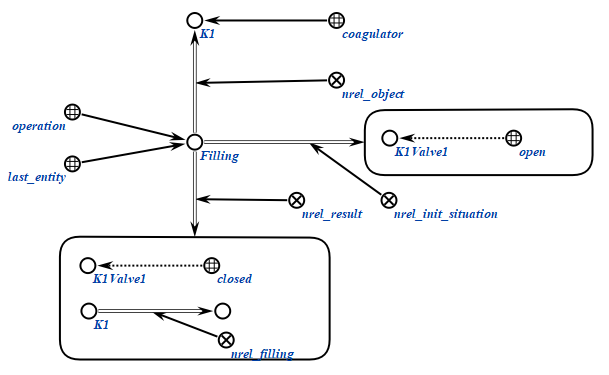
\includegraphics[width=\linewidth,height=0.68\textheight,keepaspectratio]{figures/sd_temp_entities/process_description.png}
		\end{figure}
	\end{SCn}
\end{frame}

\begin{frame}{\\Example of a complex action}
	\topline
	\justifying
	\vspace{10mm}
	\begin{SCn}
		\begin{figure}[H]
			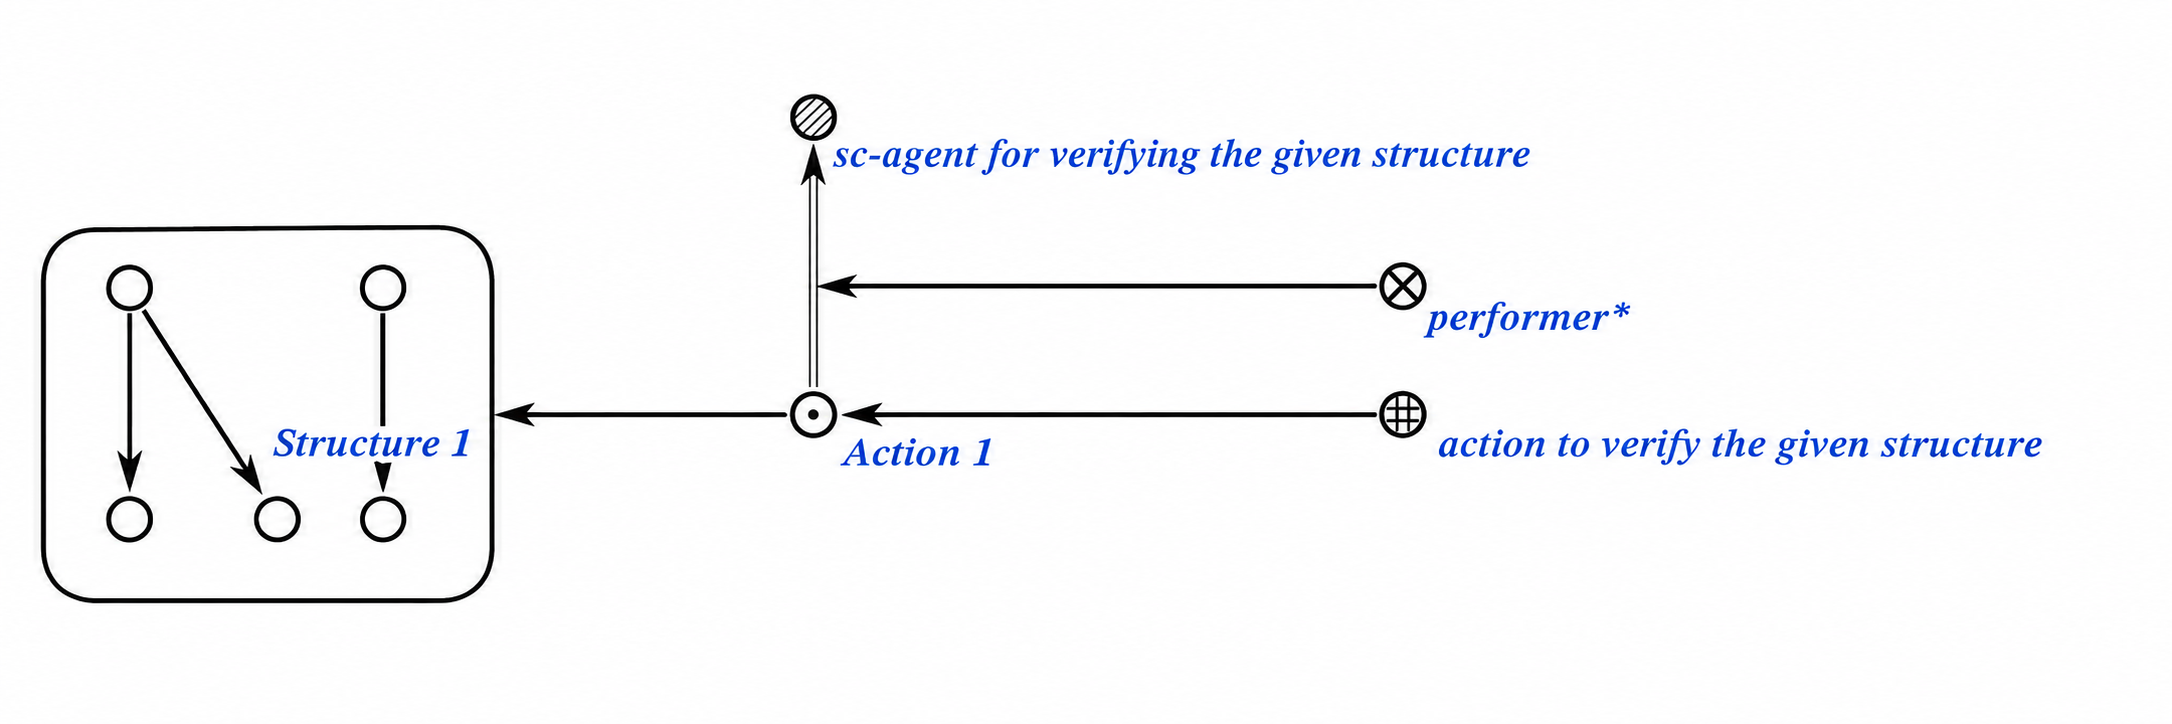
\includegraphics[width=\linewidth,height=0.68\textheight,keepaspectratio]{figures/sd_actions/actions1_en.png}
		\end{figure}
	\end{SCn}
\end{frame}

\begin{frame}{\\Example of a complex action}
	\topline
	\justifying
	\vspace{10mm}
	\begin{SCn}
		\begin{figure}[H]
			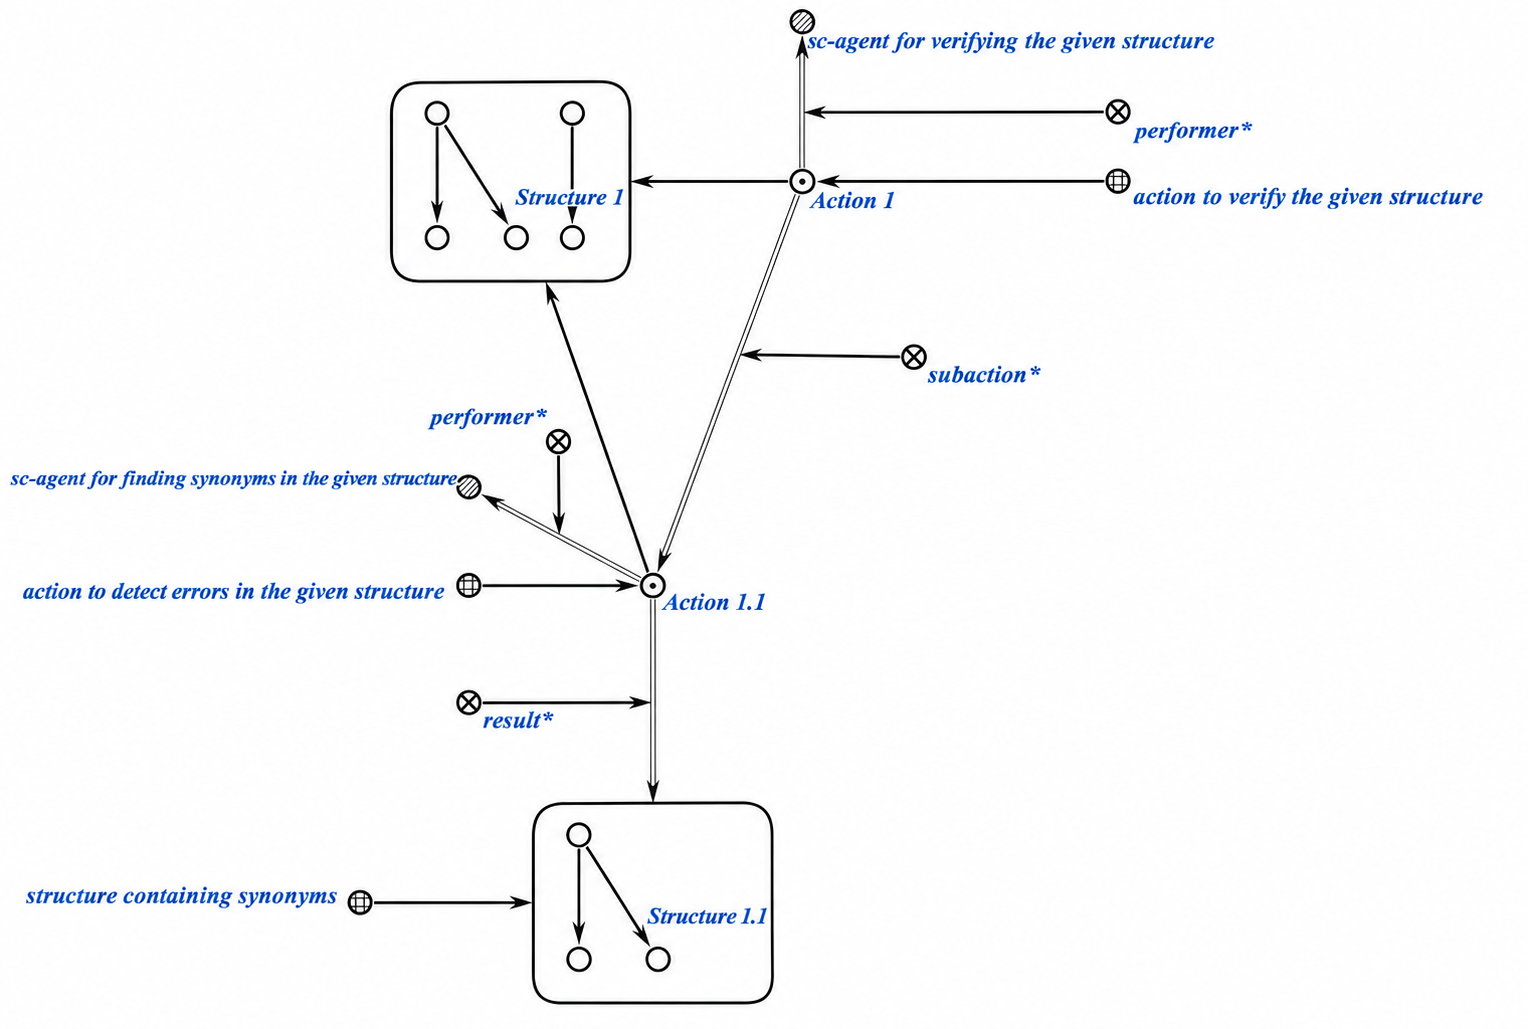
\includegraphics[width=\linewidth,height=0.68\textheight,keepaspectratio]{figures/sd_actions/actions2_en.png}
		\end{figure}
	\end{SCn}
\end{frame}

\begin{frame}{\\Example of a complex action}
	\topline
	\justifying
	\vspace{10mm}
	\begin{SCn}
		\begin{figure}[H]
			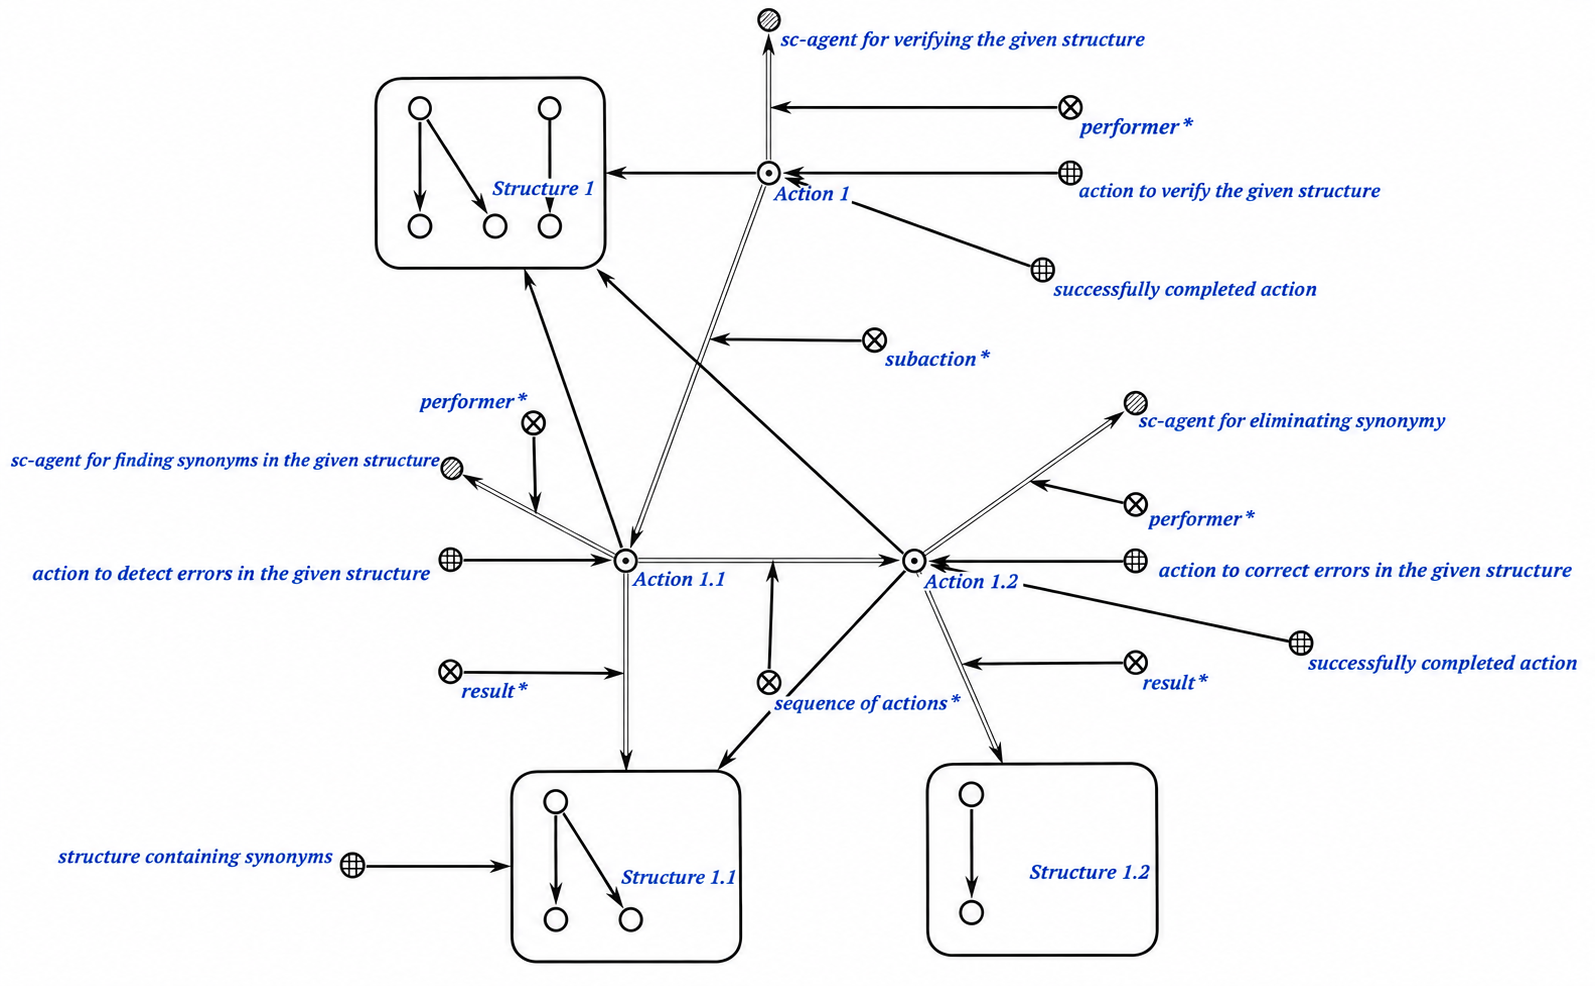
\includegraphics[width=\linewidth,height=0.68\textheight,keepaspectratio]{figures/sd_actions/actions3_en.png}
		\end{figure}
	\end{SCn}
\end{frame}
